\documentclass{article}
\usepackage{tikz}
\usetikzlibrary{decorations, calc, arrows, arrows.meta, shapes.multipart, positioning}

\begin{document}
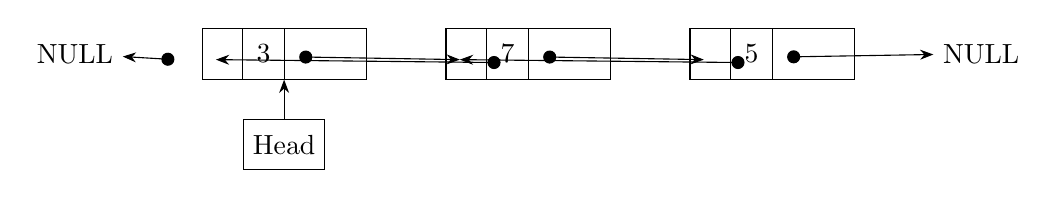
\begin{tikzpicture}[>=Stealth,
    node distance=0.5cm and 1.0cm,
    list/.style={rectangle split, rectangle split parts=3, draw, rectangle split horizontal, minimum size=18pt, inner sep=5pt, text=black}
]

% Create the nodes
\node[list] (A) { \nodepart{second} 3 \nodepart{third} \phantom{prev}};
\node[list, right=of A] (B) { \nodepart{second} 7 \nodepart{third} \phantom{prev}};
\node[list, right=of B] (C) { \nodepart{second} 5 \nodepart{third} \phantom{prev}};

% Create the NULL nodes
\node[left=of A] (null1) {NULL};
\node[right=of C] (null2) {NULL};

% Draw the pointers
\draw[*->] ([xshift=-15pt]A.text) -- (null1);
\draw[*->] (A.third) -- (B.text);
\draw[*->] (B.third) -- (C.text);
\draw[*->] (C.third) -- (null2);

\draw[<-*] (A.text) -- (B.second);
\draw[<-*] (B.text) -- (C.second);

% Draw the head pointer
\node[below=of A, rectangle, draw, minimum size=18pt] (head) {Head};
\draw[->] (head) -- (A);

\end{tikzpicture}
\end{document}
